\section*{WU4}
\begin{figure}[here]
	\center
	\caption{wu4}
	\label{fig:wu4}
	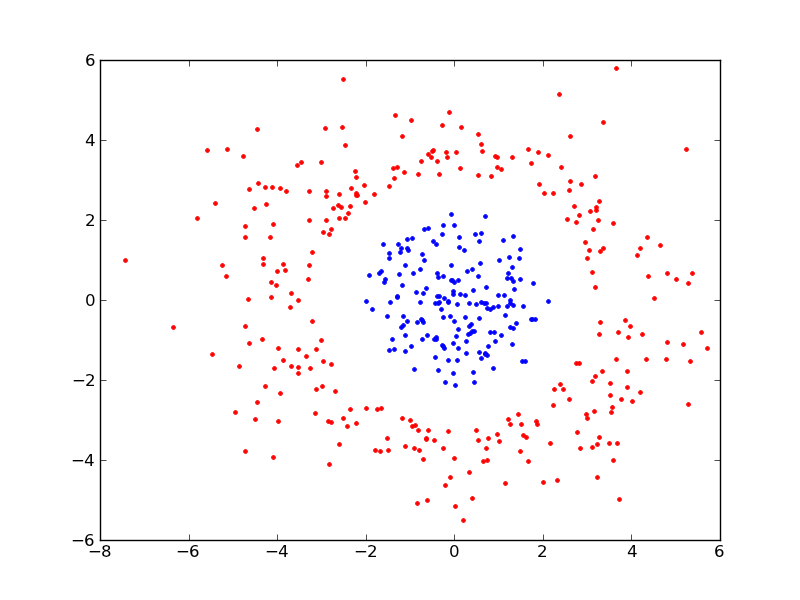
\includegraphics[width=4.0in]{img/wu4.png}
\end{figure}
Figure \ref{fig:wu4} shows the plot of the data. 
Vanilla PCA will find this data difficult because the variance in all directions is similar. This means that eigenvectors can point in any direction.

The large eigenvalues have no significance. For example, with a poly3 kernel, the eigenvalues are ridiculously 
large due to cubing the dot product. What does hold significance, however, is the normalized eigenvalues. 

\section*{WU5}
\begin{figure}[here]
\label{fig:wu5}
	\center
	\caption{wu5}
	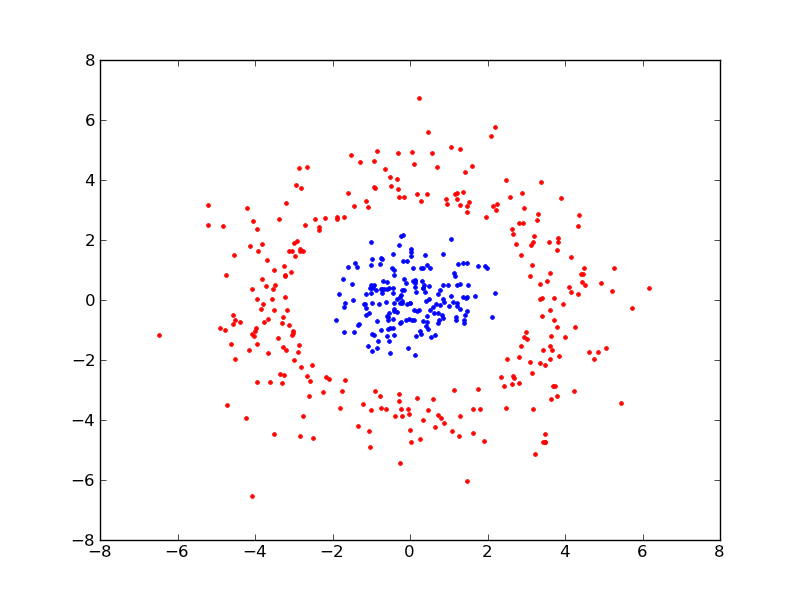
\includegraphics[width=4.0in]{img/wu5.png}
\end{figure}
Figure \ref{fig:wu5} shows the result of PCA. 
PCA did not do what we want it to do :'(
In addition to the reasons listed in WU4, vanilla PCA 
did not do what we wanted to do because the resulting data 
is not linearly separable.

\section*{WU6}
\begin{figure}[here]
	\center
	\caption{wu6}
	\label{fig:wu6}
	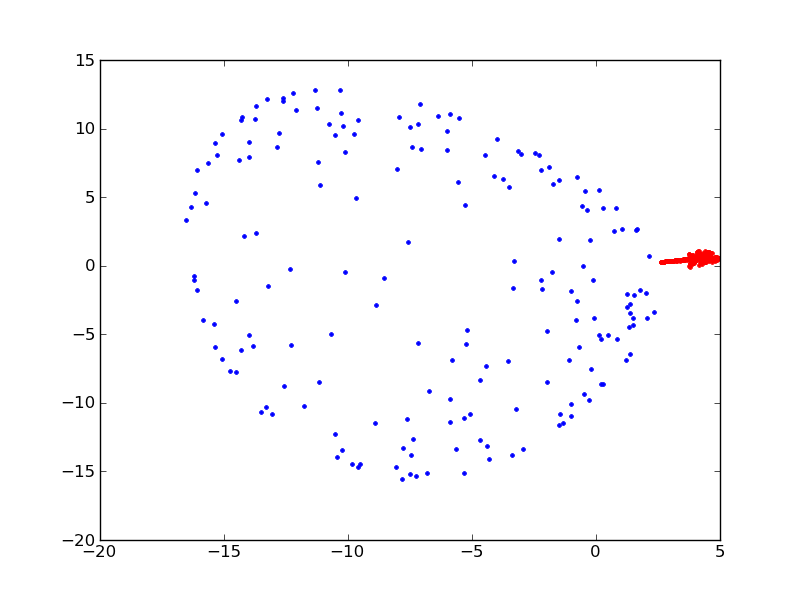
\includegraphics[width=4.0in]{img/wu7_rbf1.png}
\end{figure}

The eigenvalues for KPCA with rbf1 kernel is [ 0.08228617  0.05882765], which is significantly smaller than
the eigenvalues for KPCA with linear kernel: [ 6.00010675  5.57361851]. This means that the rbf1 kernel does a much 
better job at making the data linearly separable than the linear kernel. See the Figure \ref{fig:wu7_rbf1} for a plot of the rbf1 kernel and Figure \ref{fig:wu7_linear} for the plot of the linear kernel for a visual comparison.

\section*{WU7}
\begin{verbatim}
	linear: evals [ 6.00010675  5.57361851]
	poly2: [ 60.36960773  57.61047579]
	poly3: [ 2316.48011949  2139.88680252]
	rbf0_2: evals [ 0.15469386  0.10178237]
	rbf0_5: evals [ 0.1194342   0.06754455]
	rbf2: evals [ 0.05293176  0.04460633]
	rbf5: evals [ 0.02906865  0.02521906]
\end{verbatim}
Plots for the various kernels:
\begin{itemize}
	\item linear: Figure \ref{fig:wu7_linear}
	\item poly2: Figure \ref{fig:wu7_poly2}
	\item poly3: Figure \ref{fig:wu7_poly3}
	\item rbf0.2: Figure \ref{fig:wu7_rbf0_2}
	\item rbf0.5: Figure \ref{fig:wu7_rbf0_5}
	\item rbf2: Figure \ref{fig:wu7_rbf2}
	\item rbf5: Figure \ref{fig:wu7_rbf5}
\end{itemize}


\begin{figure}[here]
	\center
	\caption{wu7 linear}
	\label{fig:wu7_linear}
	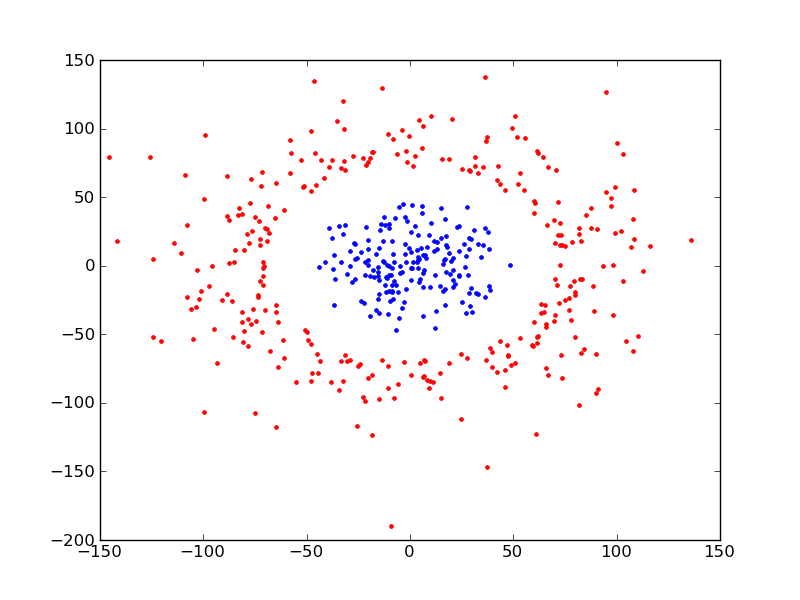
\includegraphics[width=4.0in]{img/wu7_linear.png}
\end{figure}

\begin{figure}[here]
	\center
	\caption{wu7 poly2}
	\label{fig:wu7_poly2}
	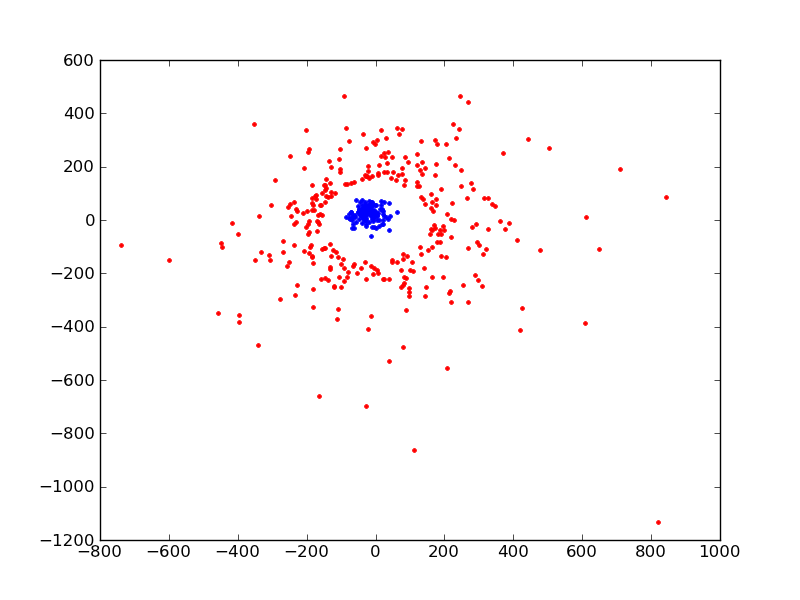
\includegraphics[width=4.0in]{img/wu7_poly2.png}
\end{figure}

\begin{figure}[here]
	\center
	\caption{wu7 poly3}
	\label{fig:wu7_poly3}
	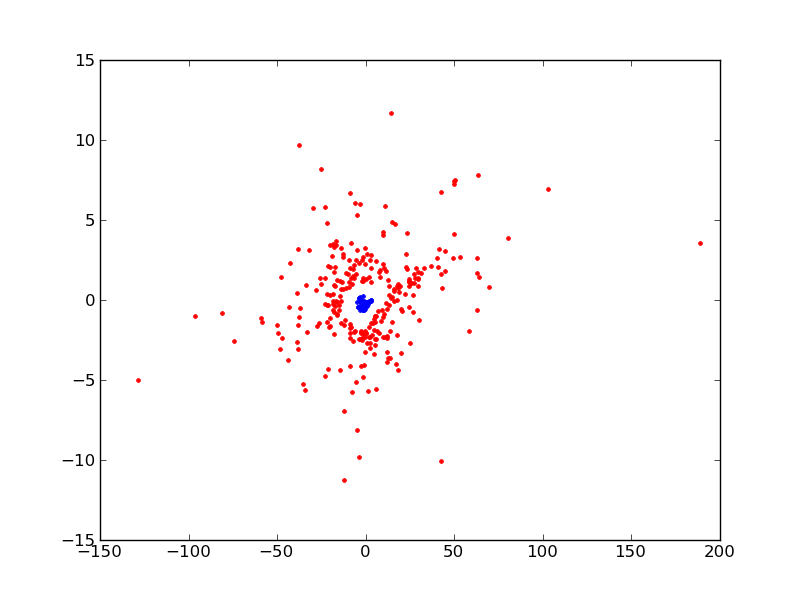
\includegraphics[width=4.0in]{img/wu7_poly3.png}
\end{figure}

\begin{figure}[here]
	\center
	\caption{wu7 rbf0.2}
	\label{fig:wu7_rbf0_2}
	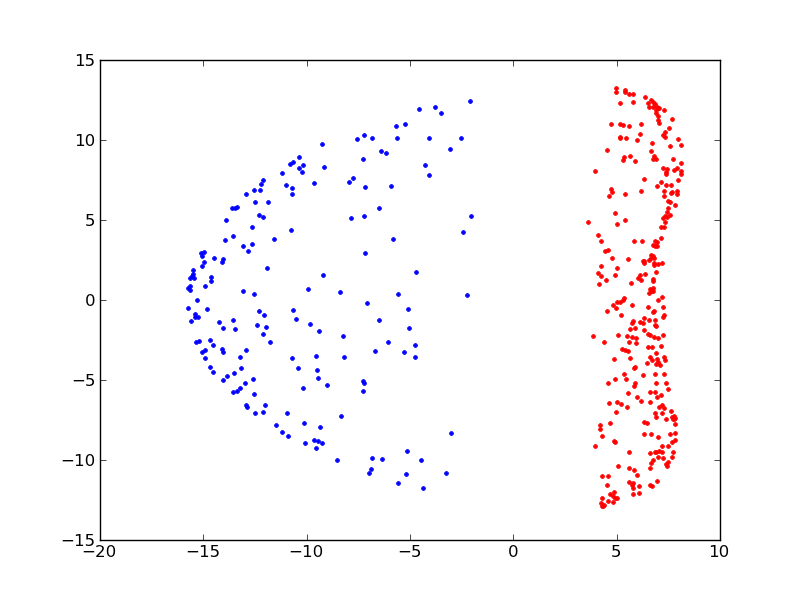
\includegraphics[width=4.0in]{img/wu7_rbf0_2.png}
\end{figure}

\begin{figure}[here]
	\center
	\caption{wu7 rbf0.5}
	\label{fig:wu7_rbf0_5}
	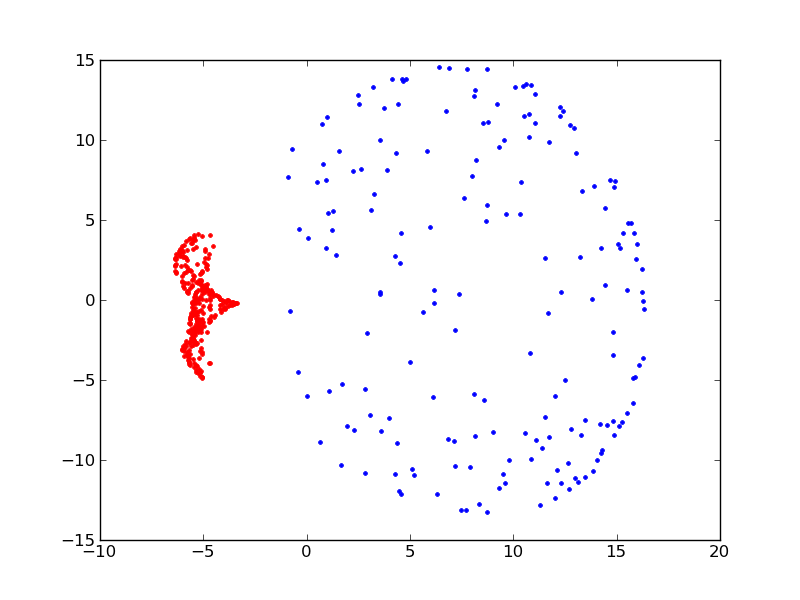
\includegraphics[width=4.0in]{img/wu7_rbf0_5.png}
\end{figure}

\begin{figure}[here]
	\center
	\caption{wu7 rbf1}
	\label{fig:wu7_rbf1}
	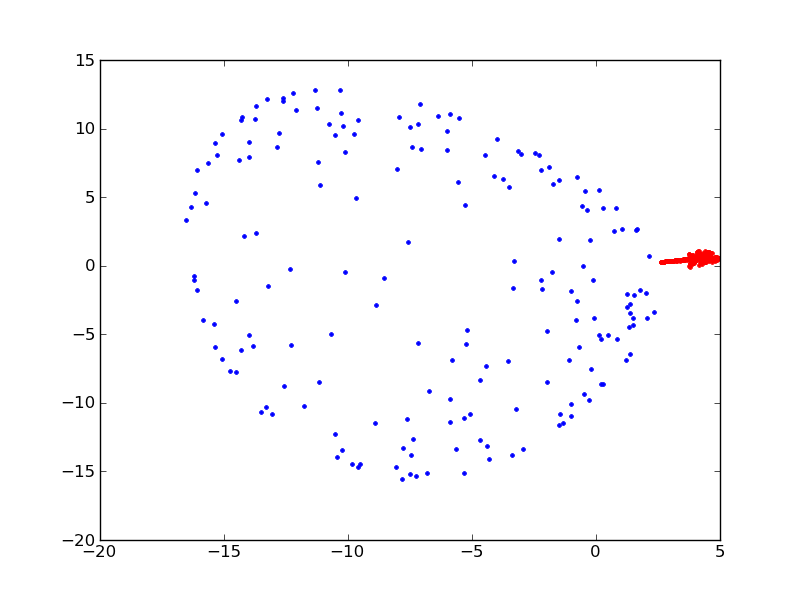
\includegraphics[width=4.0in]{img/wu7_rbf1.png}
\end{figure}

\begin{figure}[here]
	\center
	\caption{wu7 rbf2}
	\label{fig:wu7_rbf2}
	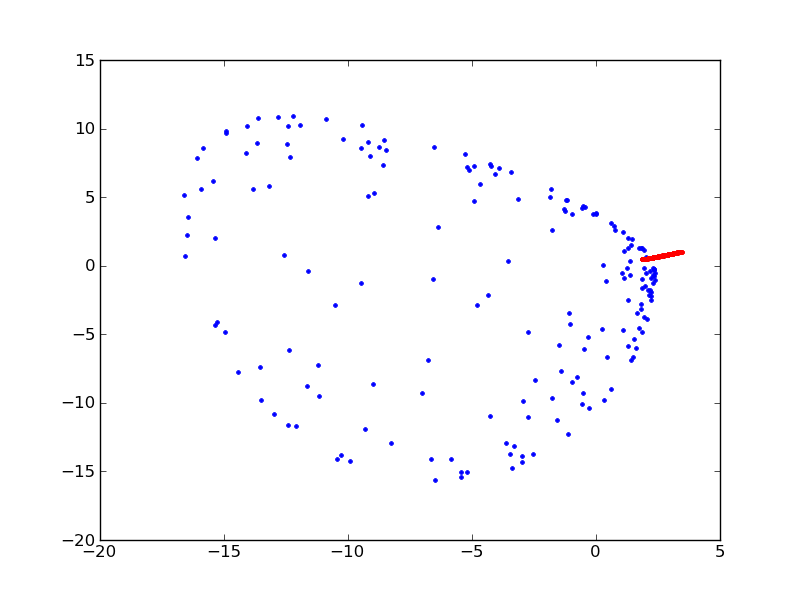
\includegraphics[width=4.0in]{img/wu7_rbf2.png}
\end{figure}

\begin{figure}[here]
	\center
	\caption{wu7 rbf5}
	\label{fig:wu7_rbf5}
	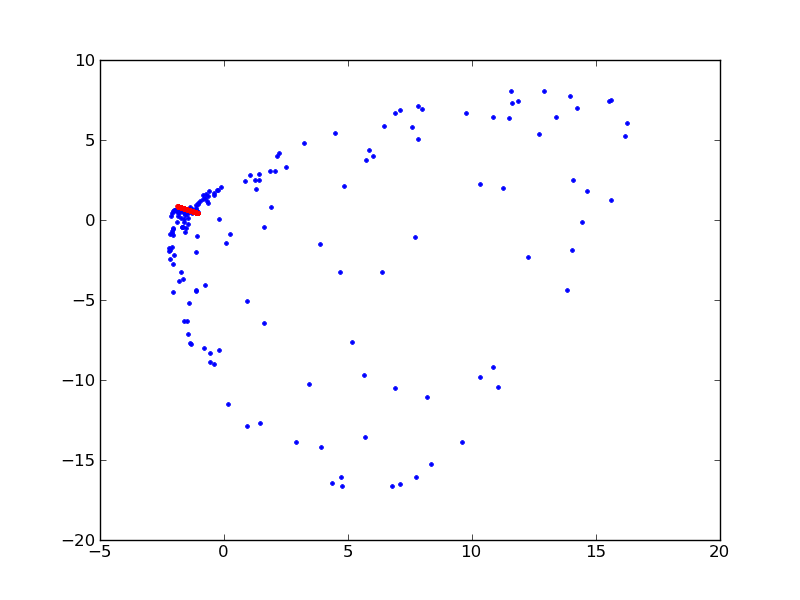
\includegraphics[width=4.0in]{img/wu7_rbf5.png}
\end{figure}